\chapter{Discussion}
\label{chp:discussion} 

\section{Introduction}

This chapter seeks to assess the implementations presented in chapter \ref{chp:implementation} based on their performance which is detailed in chapter \ref{chp:results}. The following discussions seek to qualitatively evaluate how suitable the implementations are for offshore robotic maintenance. The first section will discuss the performance of the system as a whole. Next follows a discussion on the strengths and weaknesses of the navigation and mapping systems. The chapter is concluded with a section on future work. 

\section{Overall Assessment}

The overall system, as it is at the end of this master's project, is a functioning proof of concept for a mobile autonomous robot. All planned modules were implemented. Some of these, however, are only capable of demonstrating basic functionality and the possibility of more robust and complete implementations. The most important features, camera based mapping and navigation, were successfully implemented and configured. The current implementations leaves much room for further improvements in terms of robustness, parameter tuning, functionality and ease of use.

\subsection{Choice of Development Tools}

Using \ac{ROS} as a development framework might have been the most important factor that contributed to a functional solution. In the end, \ac{ROS} proved to be a flexible and rich tool, despite its novel structure and initial learning curve. Experienced users of \ac{ROS} will most likely be able to rapidly implement and test robot concepts.  Since its inception in 2007, \ac{ROS} has become a mature and rich set of tools and functionality packages that anyone can implement and develop further. Further development by users is even encouraged by many of the \ac{ROS} package creators. The node structure in \ac{ROS} is also a good way of structuring the entire system into self contained, manageable and reusable modules. This makes it easier to reuse parts of this implementation in later projects, and will hopefully benefit ensuing projects on this topic.

\subsection{Assessment of Prototype Design}

Roughly estimated, the robot prototype have travelled a distance of approximately $1km$ during the master's project. Of these, roughly $100-200m$ were driven in autonomous mode. The bulk of these distances were accomplished over a period of 3 intensive days, while the rest was spread throughout the last third of the semester. Time available for testing was somewhat reduced as a consequence of breakdowns or depleted batteries. Another cause of the delays are caused by \ac{EMC} issues between the motor control card (A3BU) and the AC inverters. It has not been made clear if the problem is caused by only one or both of the inverters. It was possible to increase the immunity of the motor control card by grounding it to the robot chassis. The current grounding connection is not reliable at this time.

So far, the robot prototype has been developed for a few specific functionalities, and coexistence between the robot systems has not been a priority. Future projects could benefit from a comprehensive and long-term approach towards designing a maintenance robot. The following paragraphs will go through some specific design choices on the current robot, and discuss potential shortcomings. 

\subsubsection{Suboptimal Power Supply}

Some time was spent on building a new rear compartment to house the various robot equipment, including the battery and both on-board computers. For internal power, the robot uses a 12 V car battery as a power source. Figure \ref{fig:sensor_connections} and \ref{fig:power} highlights the inefficient power supply layout. The Kinect requires a supply of 12V DC, which is supplied from an adapter plugged into a 230V AC source. Receiving 12 V directly from the battery might be a more efficient solution.

\subsection{Success and Quality of the ROS Integration}

Integrating and configuring \ac{ROS} with the existing robot was the most time consuming task of this project. The current implementation is capable of autonomous navigation and long-term map building. Remote operation from the \ac{OCS} and Android device is also possible. A major shortcoming of the current configuration is the lack of usability. The current system is 
cumbersome and difficult to use. A potential difficulty may be to separate the parts that work well from the more unstable parts of the system. 


\section{Assessment of RTAB-Map}

The mapping session results demonstrated both strengths and weaknesses  in the chosen mapping method, \ac{RTAB-Map}. The results show that multi session mapping works rather well if the conditions are favorable, e.g. in environments with a sufficient amount of detectable visual features. 

\subsection{Quality and Thoroughness of the Tests}

\ac{RTAB-Map} was tested in a diverse set of indoor environments as well as in the simulated ''Asphalt'' world in Gazebo. A significant shortcoming of these tests was the lack of testing and comparison of different parameter settings for the method. Further parameter tuning and better mapping techniques could have benefited the mapping performance.

Another shortcoming is the small number of live mapping trials. Configuring and learning to use the mapping system was a time consuming process. Problems with the robot hardware and the environment itself gave rise to additional delays. The laptop running \ac{ROS} and the on-board car battery had to be recharged periodically, which took a considerable amount of time. The live loop closure tests were carried out at times when a lot of students were moving through the hallways. These factors made it difficult to perform comparable tests, and proved to be a complicating factor for the appearance based mapping system. 

A third weakness in these trials is that the system was tested with only one sensor configuration. \ac{RTAB-Map} can utilize both a RGB-D camera, a LIDAR and odometers, but these tests were only carried out with the Kinect and the LIDAR.

Simulation in Gazebo has been an invaluable option throughout the project. However, the inherent difference between the real and the simulated world should be discussed. A poorly designed simulator world could call into question whether the simulated results are representative for the mapping performance. A notable difference between the real and simulated trials, which should be kept in mind when reading the next subsection, is the how feature rich the simulated floors are. This will become apparent when the reader compares how the feature detectors extracts features. In the recorded material bundled with this thesis, it is apparent that the simulated floor is very feature rich compared to the real world floor. In retrospect, a simulated world with a simpler floor texture might have served this project better than \texttt{asphalt.world}. 

The developers of \ac{RTAB-Map} have created several datasets which can be used to reproduce their results and tune the mapping system. One such dataset, from the computer game ''Need for Speed: Most Wanted'', shows that \ac{RTAB-Map} does work in a simulated environment\footnote{RTAB-Map: NFSMW data set (part 1): \url{https://www.youtube.com/watch?v=kghs6XM8Yzw}}. 


\subsection{Weaknesses}
\label{sec:weaknesses_mapping}
Appearance based loop closure detection with \ac{RTAB-Map} has many confirmed and potential weaknesses that must be addressed. Figure \ref{fig:gazebo_lc_features} from a simulator session illustrates an incorrect loop closure detection with a subsequent incorrect odometry correction of the previously visited locations. The figure shows that the matched features are based on the ground plane in the simulated world. Having a feature rich ground plane could be a weakness with the simulated world, as it is not was not a good analogue to the real world. The depth map generated by the Kinect was in fact quite sparse at the ground plane. Another error that occurred during simulations is incorrect merging of two maps of the same area (figure \ref{fig:Incorrect_lc_detection}). This particular event was caused by having two very similar locations in the same area. 

A potential problem is that the appearance of the environment will change based on the time of day, time of year and potential wear and tear on the surroundings. How robust the feature detectors (\ac{SIFT}, \ac{SURF}, \ac{ORB} etc.) are to such changes was \textit{not} investigated during this project.  

\subsection{Strengths}

\ac{RTAB-Map} is packed with features, parameters and useful tools. It supports many sensor configurations, including stereo cameras. The \ac{ROS} wrapper makes it easy to integrate the method into an existing robot system. The developer or user has access to hundreds of parameters to tailor and fine-tune the mapping system. Object recognition and 3D obstacle detection is also useful features that will support a maintenance robot. 

Another strength is that \ac{RTAB-Map} works with any RGB-D sensor. It might be possible to to use both an active camera and a stereo camera, and switch between the two, based on the conditions. A stereo camera is better suited for outdoor mapping than a Kinect, due to the presence of IR wavelengths in sunlight. 


\subsection{Suitability For Robotic Maintenance}

\ac{RTAB-Map} has a wealth of configuration options with many capabilities that can make it suitable for a remotely operated and autonomous maintenance robot. The built-in object recognition capabilities are useful. Unfortunately, the object recognizer was not tested. 

As mentioned in section \ref{sec:weaknesses_mapping}, it is clear that an appearance based method may be vulnerable to natural variations in the environment. This fact could completely rule out \ac{RTAB-Map} as an outdoor \ac{SLAM} system. The suitability of the method will also depend on the robots intended task. Based on the discussion so far, it may seem that \ac{RTAB-Map} can be useful for an indoor robot during normal operation of the facility. 

Section \ref{sec:robotizing_offhsore_maintenance} discussed the hazards of offshore \ac{OG} production and how a robot could respond to crisis situations such as hydrocarbon leaks, toxic gases or fires. Such events could alter the appearance of the environment, which in turn may knock out the \ac{SLAM} capabilities a robot.

\section{Navigation}

Integrating the \ac{ROS} navigation stack into a new mobile base was in itself a fairly simple procedure. Finding a good configuration turned out to be a more complicated process. Navigation was tested on both the simulator and the live robot. It became apparent during the testing sessions that the behaviour of the simulated robot was not analogue to the real robot. Recall that the simulated robot is controlled by a slip steering plugin in Gazebo, while the real robot is closer to a differential drive vehicle. In addition, the motor control in the real robot is an open loop system. The wheel commands from \ac{ROS} will normally result in a lower linear velocity and yaw rate. A consequence of this discrepancy between the real and simulated robots, is that the performance assessment of navigation stack in the simulator will have a reduced weight.

\subsection{The Tuning Process}

There are no official tuning strategies for the navigation stack in \ac{ROS} besides a basic guide. The guide serves to give users a general idea of where to start and what to check\cite{ROS_navigation_tuning}. The tuning process is currently a ''change and check'' process, partially based on guesswork or of copying similar solutions from other projects. This is far from ideal, as it is both time consuming and a hindrance for finding an optimal solution. 

It should be noted that the navigation stack has been thoroughly tested on robots with square or circular bases. The highly rectangular base ($80cm \times 37cm$) on this robot may have been a handicap. 



As with the \ac{SLAM} test sessions on the live robot, the cumbersome hardware and limited battery life significantly constrained the amount of time available for testing of the navigation stack. 



\subsection{Performance}

Live testing showed promising results, despite a few quirks. The live robot would reliably plan a path to a goal location and move the base to this location, given that the goal was feasible. Sometimes, the robot would stop a few centimetres before reaching the goal location.

Based on the test results, the live robot should have a higher minimum speed setting than the simulated robot in order to overcome friction and other resisting forces. The reason for this is that the velocity command is matched against wheel speeds when the robot is off the ground, i.e. the wheels are spinning freely. If the motor control card is expanded with a speed regulator, the minimum speed may be reduced.

\section{Suitability for Offshore Maintenance}

This is just a prototype. Mobility issues.
Kinect-like sensors and ROS could be useful. It is at least an excellent tool for ''rapid'' prototyping.

The current configuration has many shortcomings as a maintenance robot. In its current form, it is more suitable to test various technologies and concepts. 

The current sensor configuration is set up to facilitate testing of \ac{SLAM} and navigation.

\subsubsection{Current Design and Robotic Maintenance}
\label{sec:design_maintenance}
A typical offshore installation floor will most likely be made of steel and steel gratings with many holes, gaps and sharp edges\cite{graf2008mobile}. The current mobile base is better suited for completely even surfaces, and would benefit greatly for a more rugged set of wheels. \cite{graf2008mobile} is also referring to a minimum size for passage ways that could serve as guidelines for later prototypes. The suggested minimum workspace boundaries, $0.75m$ wide and $1.5m$ high corridors, imply that the prototype used in this project is too big, given its footprint of $80cm \times 37 cm$. Another problem is that the Kinect would have trouble with mapping and navigating in this environment, given its measured minimum range of $0.5m$, not to mention the reliable minimum depth of $0.8m$. In this autors's specialization project\cite{lindrup}, the minimum measurable depth of the obstruction detection was found to be $\approx 40 cm$. The minimum range was limited by the maximum disparity parameter. Increasing the detectable maximum disparity could reduce the detectable range even further, thus making it a better option for narrow spaces where depth ranges are short. 

As the motor control card is an open loop system, slopes and increased friction for whatever reason will affect the speed of the mobile base. This may cause the base to slow down, speed up or even stop completely if it is driving up a slope that is too steep.

Given that the navigation stack in \ac{ROS} is thoroughly tested on square or circular bases, designing a new base to be either square or circular could increase the robustness of the navigation system. A holonomic drive could also make the robot more maneuverable, which may be useful in tight spaces.

The current design of the mobile base is struggling to support the weight of the robot. The small wheels are struggling with small obstacles such as door thresholds or floor gaps in the entrance to elevators. \ac{MIMROex}, a comparable robot, is equipped with a variant of a differential drive base with larger wheels suitable for driving over steel gratings and slippery surfaces.



\subsection{The Kinect}

As mentioned in section \ref{}, the Kinect is an active sensor that measures depth by projecting an infra red speckle pattern onto the surroundings.  Kinect for Xbox 360 can't be used in commercial applications because of its license. There are, however, similar sensors that can replace the Kinect.

\subsection{Open Source Software and Security}

\ac{ROS} and other open source projects thrive on active communities of contributors. Both \ac{PCL} and \ac{ROS}, as well as many other libraries and frameworks, are built on a collaborative effort from researchers and developers across the globe. This is open structure is great for speeding up innovation. Issues and bugs can also be discovered more quickly by anyone. Another benefit is that every detail in an open source project is open for scrutiny by those who want to use it. This is also a problem in terms of security. While anyone can find bugs and issues, the code is also open to those who are looking for possible exploits and vulnerabilities. If a system is targeted for sabotage, and it is widely known that the system uses open source software, it might be more vulnerable to security threats.

\section{Future Work}

\subsection{Autonomous Non-Destructive Testing}

Advancements in \ac{AI}, big data and machine learning opens up exciting possibilities for autonomous \ac{NDT}. Branches of this technology is usually encountered in the context of image recognition, i.e. teaching machines to understand what they see. The same concepts may be applied to forms of \ac{NDT} besides regular visual sensor input, such as ultra sound or eddy currents for corrosion detection.  

\subsection{Large Scale Kinect Fusion - Kintinous}

Kinect Fusion has great potential for augmented reality. Augmented reality is a concept which blends the real and virtual environment. This opens up opportunities to create realistic and immersive training scenarios for the operators. Unfortunately, Kinect Fusion is limited reconstructing a rather small volume depending on the resolution. By varying the resolution, volumes can at the least cover a normal office desk and at the most cover a small room \cite{keylist}.  

Kintinous...

A guide on how to build Kintinous can be found  at \href{Github}{https://github.com/mp3guy/Kintinuous}. The procedure is complicated, as it usually is for experimental builds. It is recommended to attempt the procedure on a fresh install of Ubuntu 14.04 or 15.04 \cite{Kintinous}.

\subsubsection{Improve the Communication Protocols}

Communication between \ac{ROS} and the XMEGA A3BU, the Bluetooth device and the \ac{OCS}, all use the same pattern: A start byte \texttt{'':''}, the message with the speed setting and a stop byte \texttt{''Esc''}. In later projects, it could be beneficial to implement a more robust and rich communication protocol with more options for remote operation. 

\subsubsection{Implement a Fully Functional Operator Control Station}

At the end of this project, the \ac{OCS} provided functionality for moving the robot, and displaying live video from the Kinect. 

\subsection{Hardware}

Several hardware-related issues became apparent over the course of the project - especially toward the final weeks. These issues are likely the results of many disconnected projects on the same hardware.

\subsubsection{Kinect Sensor Location}

This is the first semester in which a Kinect has been used on the robot. At the moment, the sensor is placed directly over the \ac{LIDAR} device. Because the depth sensor in the Kinect for XBOX 360 has a minimum range of roughly $0.5 m$, it cannot detect objects within reach of the robot arm. It is recommended to find a new location further back on the robot. 

\subsubsection{Combine Stereo Cameras with Kinect-like Sensors}

As mentioned, both active and passive depth cameras have limitations. The Kinect does function in direct sunlight, but it can measure depth in the dark. Passive depth sensors, for example stereo cameras, does depend on visible light to sense anything at all. While RTAB-Map does depend on visibility for loop closure detection, there are  other \ac{SLAM} methods, e.g. \textit{Kinect Fusion}, which do not. An implementation could use a light sensor to sense light that may interfere with the Kinect. Light levels could be compared to a threshold and switch between the stereo cameras or the Kinect depending on how well each sensor will work in the current conditions. 

\subsubsection{On-board Computer Suitable for Moving Platforms}

Because this author used his own computer to control the robot, all features related to \ac{ROS} was removed from the robot at the end of the project. A new computer should be equipped with \ac{SSD} storage

\subsubsection{Wheels}

\begin{wrapfigure}{r}{0.5\textwidth}
	\vspace{-20pt}
	\begin{center}
		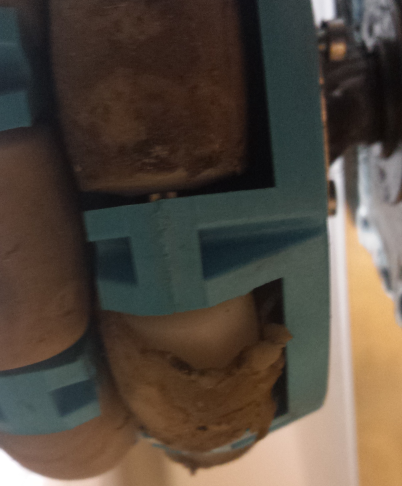
\includegraphics[width=0.48\textwidth]{worn_wheel2}
	\end{center}
	
	\caption{Worn omniwheel}
	\label{fig:worn_wheel}
	%\vspace{-20pt}
\end{wrapfigure}

There were mainly two issues with the omni-wheels this semester: They are worn out, and one wheel slipped out of the motor drive shaft. The rubber on a few of the perpendicular rollers is loose and about to fall off the plastic rims. This causes the robot to shake, which can damage spinning hard disk drives or shake the sensors out of their calibrated positions.   

A new set of wheels should be able to carry the weight of the robot, and enable the robot to drive over small barriers such as door sills and steel grates. This will most likely prompt a redesign of the mobile base.